\section{Are these theories renormalizable?}
\label{sec:renorm}

A quantum field theory is \emph{renormalizable} if the divergences of its perturbation theory can be
removed by adjusting finitely many parameters of its Lagrangian. The test is power counting. In
$D+1$ space-time dimensions (with $D$ the number of space dimensions) the action is dimensionless, so a
fermion field has the mass dimension $[\Psi_{\rm LL}]=D/2$, a scalar field $[\phi_{\rm LL}]=(D-1)/2$, and
the couplings have
\begin{equation}
[G_{\rm LL}]=1-D,\quad [g^{\rm Y}_{\rm LL}]=\tfrac{3-D}2,\quad [\lambda^{(1)}_{\rm LL}]=[\lambda^{(2)}_{\rm LL}]=3-D
\label{eq:dims}
\end{equation}
for the contact interaction of Eq.~(\ref{eq:ham}), a Yukawa coupling of a scalar to two fermions, and a
quartic coupling of scalars (R-1). A coupling of negative mass dimension makes a theory
non-renormalizable: for $D=3$ the contact coupling has $[G_{\rm LL}]=-2$, while the Yukawa and quartic
couplings are dimensionless; for $D=7$---the $7+1$ manifold, and the $4+4$ manifold, where power
counting sees the total dimension 8---all of them have negative dimension ($-6$, $-2$, $-4$).

\subsection{Power counting}

A one-particle-irreducible graph with $n^{\rm v}_{\rm LL}$ vertices, $n^{\rm int,F}_{\rm LL}$ internal
fermion and $n^{\rm int,B}_{\rm LL}$ internal boson lines has $n^{\rm loop}_{\rm LL}=n^{\rm int,F}_{\rm
LL}+n^{\rm int,B}_{\rm LL}-n^{\rm v}_{\rm LL}+1$ loops, and, since a fermion propagator falls like the
inverse momentum and a boson propagator like its square, the \emph{superficial degree of divergence}
\begin{equation}
\deg_{\rm LL}=(D+1)\,n^{\rm loop}_{\rm LL}-n^{\rm int,F}_{\rm LL}-2\,n^{\rm int,B}_{\rm LL}.
\label{eq:deg}
\end{equation}
Eliminating the internal lines with the number of line ends at the vertices gives, for the contact theory
and for the theory with Yukawa and quartic vertices,
\begin{align}
\deg_{\rm LL}&=(D+1)-\tfrac D2n^{\rm ext,F}_{\rm LL}+(D-1)\,n^{\rm v}_{\rm LL},\label{eq:degc}\\
\deg_{\rm LL}&=(D+1)-\tfrac D2n^{\rm ext,F}_{\rm LL}-\tfrac{D-1}2n^{\rm ext,B}_{\rm LL}\nonumber\\
&\quad+(D-3)\big(\tfrac12n^{\rm v,Y}_{\rm LL}+n^{\rm v,4}_{\rm LL}\big),\label{eq:degy}
\end{align}
with $n^{\rm ext,F}_{\rm LL}$, $n^{\rm ext,B}_{\rm LL}$ the external fermion and boson lines and
$n^{\rm v,Y}_{\rm LL}$, $n^{\rm v,4}_{\rm LL}$ the Yukawa and quartic vertices; check R-2 compares both
formulas with the direct count on all graphs with up to six vertices. For $D=3$ the degree of the
contact theory grows by 2 with every vertex: infinitely many counterterms are needed. The degree of the
Yukawa theory does not depend on the vertices: only the finitely many functions with $\deg_{\rm
LL}\ge0$ diverge. For $D=7$ both grow (Fig.~\ref{fig:renorm}(a)).

\subsection{The contact theory needs a cutoff}

At a fixed physical gap the bare coupling that solves the gap equation~(\ref{eq:gapeq}) must vary with
the cutoff as $G_{\rm LL}\Lambda_{\rm LL}^2/(2\pi^2)\to1$: the value is {{GEN:contact_running_128}} at
$\Lambda_{\rm LL}=128$ ($\Delta_{\rm LL}=0.05$, $\mu_{\rm LL}=0.5$, $m_{\rm LL}=0.2$; R-3,
Fig.~\ref{fig:renorm}(b)). The cutoff cannot be removed by a finite number of logarithmic counterterms;
like the model of Nambu and Jona-Lasinio~\cite{NambuJonaLasinio1961}, the contact theory is an
effective theory valid below $\Lambda_{\rm LL}$.

\subsection{The Yukawa completion}

Replace the contact interaction by a complex isospin-triplet pair field $\phi_{\rm LL}=(\phi^1_{\rm
LL},\phi^2_{\rm LL},\phi^3_{\rm LL})$, a scalar of mass dimension 1 for $D=3$, with kinetic and mass
terms, the Yukawa coupling $g^{\rm Y}_{\rm LL}$ to the pairs $\Psi^T_{\rm LL}\mathsf K^\iota_{\rm LL}\Psi_{\rm
LL}$ (plus the Hermitian conjugate), and quartic self-couplings. Below the mass of $\phi_{\rm LL}$ its
exchange reproduces the contact interaction. The one-loop self-energy of $\phi_{\rm LL}$ is, up to the
constant factor of the traces over the Dirac and isospin indices, the Euclidean bubble
\begin{align}
I^{\rm bub}_{\rm LL}={}&\int_{k^{\rm E}_{\rm LL}<\Lambda_{\rm LL}}\!\frac{d^4k^{\rm E}_{\rm LL}}{(2\pi)^4}\nonumber\\
&\times\frac{k^{\rm E}_{\rm LL}\cdot(k^{\rm E}_{\rm LL}+p^{\rm E}_{\rm LL})+m_{\rm LL}^2}{[(k^{\rm E}_{\rm LL})^2+m_{\rm LL}^2][(k^{\rm E}_{\rm LL}+p^{\rm E}_{\rm LL})^2+m_{\rm LL}^2]}
\label{eq:bubble}
\end{align}
with the loop momentum $k^{\rm E}_{\rm LL}$ and the external momentum $p^{\rm E}_{\rm LL}$. Its value at
$p^{\rm E}_{\rm LL}=0$ grows like $\Lambda_{\rm LL}^2$ and is absorbed by the mass counterterm of
$\phi_{\rm LL}$; its momentum dependence grows like the logarithm of the cutoff, $d[I^{\rm bub}_{\rm
LL}(p^{\rm E}_{\rm LL})-I^{\rm bub}_{\rm LL}(0)]/d\ln\Lambda_{\rm LL}\to-(p^{\rm E}_{\rm LL})^2/(16\pi^2)$, and
is absorbed by the wave-function counterterm: the computed slope is {{GEN:bubble_slope}} against
{{GEN:bubble_target}} (ratio {{GEN:bubble_ratio}}; $p^{\rm E}_{\rm LL}=1$, $m_{\rm LL}=0.5$; R-4,
Fig.~\ref{fig:renorm}(c)). The list of renormalizable couplings is finite: besides $g^{\rm Y}_{\rm LL}$
and the masses, the quartic polynomials of $\phi_{\rm LL}$ invariant under isospin form a space of
dimension exactly 2, spanned by $(\phi^\dagger_{\rm LL}\phi_{\rm LL})^2$ and $\lvert\phi^T_{\rm
LL}\phi_{\rm LL}\rvert^2$ (R-5), with the couplings $\lambda^{(1)}_{\rm LL}$ and $\lambda^{(2)}_{\rm LL}$.

\subsection{Does non-associativity change the answer?}

No. A Lagrangian is built from fields on which the symmetry acts linearly, and a linear action of the
loop generates a Lie group (Sec.~\ref{sec:manifolds}). Check R-6 makes this precise for the simplest
case: the quadratic forms on $\mathbb B_{\rm LL}$ that are invariant under the 14 left multiplications
$L^{\rm LL}_{\mathbf x}$ and those invariant under their 56-dimensional Lie closure $\mathfrak{so}(8,\mathbb
C)$ form the same two-dimensional space, spanned by $\mathrm{Re}\,N_{\rm LL}$ and $\mathrm{Im}\,N_{\rm LL}$.
Every counterterm that the closure allows the loop allows, and conversely; power counting is unchanged.

\emph{Verdict.} In $3+1$ dimensions the spin-zero spinor superfluid of the super-loop is described by a
renormalizable theory in its Yukawa form; its contact form is non-renormalizable and needs the cutoff.
On the $7+1$ and $4+4$ manifolds every form is non-renormalizable. The non-associativity of the
super-loop neither causes nor cures this.

\begin{figure*}[t]
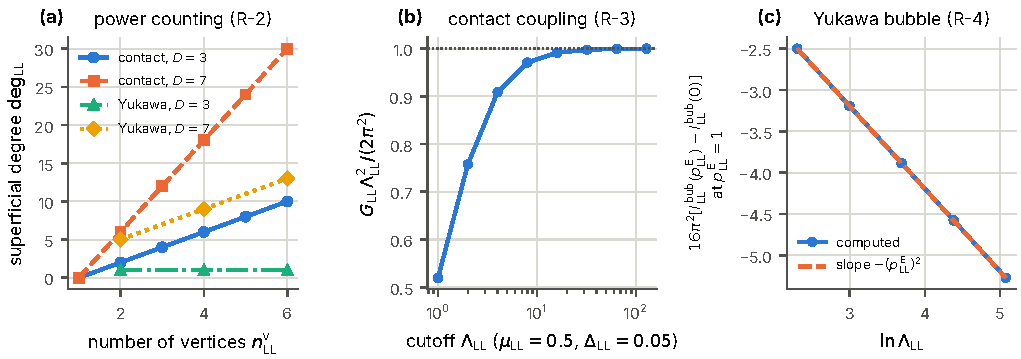
\includegraphics[width=\textwidth]{../figures/fig_sl_renorm.pdf}
\caption{Renormalizability. (a) The superficial degree of divergence of the four-fermion function of
the contact theory and of the fermion self-energy of the Yukawa theory versus the number of vertices,
Eqs.~(\ref{eq:degc}) and~(\ref{eq:degy}), for $D=3$ and $D=7$ (R-2). (b) The bare contact coupling at a
fixed gap versus the cutoff (R-3). (c) The momentum-dependent part of the bubble~(\ref{eq:bubble})
versus $\ln\Lambda_{\rm LL}$, with the slope $-(p^{\rm E}_{\rm LL})^2/(16\pi^2)$ (R-4).}
\label{fig:renorm}
\end{figure*}
